Bahan dan peralatan yang digunakan dalam pengerjaan tugas akhir ini terdiri dari perangkat keras, perangkat lunak, dan alat ukur sebagai berikut.

\subsection{Perangkat Keras}

\subsubsection{Mobil Listrik Omoda E5}

\begin{figure}[H]
    \centering
    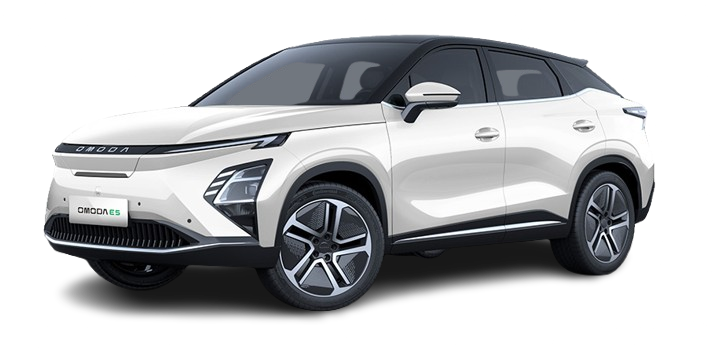
\includegraphics[width=0.6\textwidth]{gambar/omoda.png}
    \caption{Kendaraan listrik Omoda E5 yang digunakan sebagai platform pengujian.}
    \label{fig:omoda_e5}
\end{figure}

Platform pengujian yang digunakan adalah kendaraan listrik Cherry Omoda E5 dengan sistem penggerak roda depan, tenaga 204 HP, dan torsi 310 Nm.
Kendaraan ini dilengkapi dengan \emph{Advanced Driver Assistance System} (ADAS) yang menyediakan komunikasi CAN FD untuk membaca data sensor kendaraan dan mengirim perintah kemudi serta pedal gas.
Kendaraan dioperasikan dalam mode otonom melalui antarmuka CAN bus yang dikendalikan oleh komputer utama.

\subsubsection{Kamera Leopard LI-IMX390-GMSL2-120H} 

\begin{figure}[H]
    \centering
    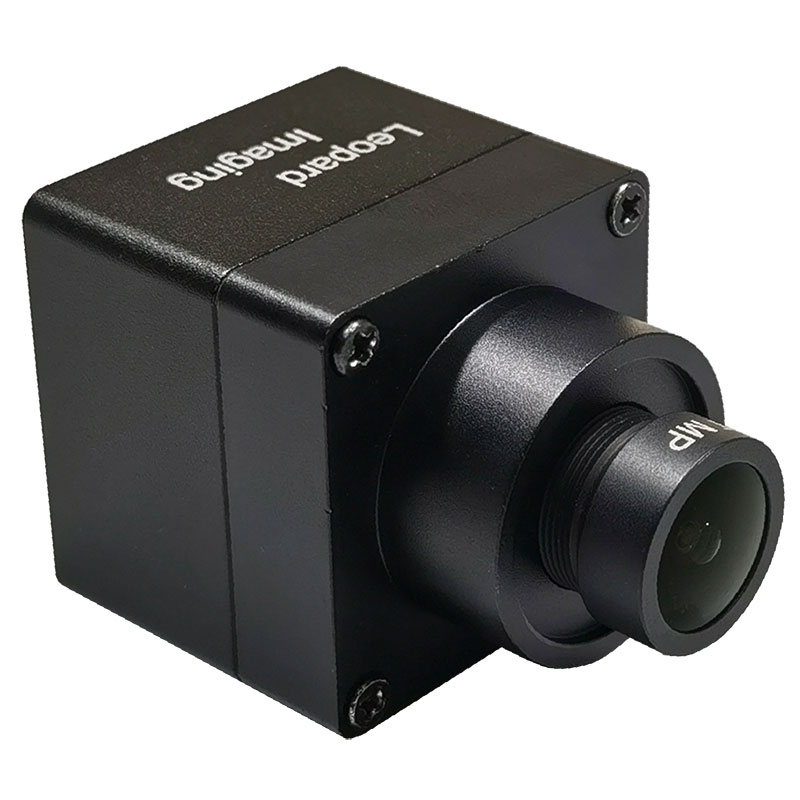
\includegraphics[width=0.3\textwidth]{gambar/leopard.jpg}
    \caption{Kamera Leopard yang digunakan untuk akuisisi citra jalan.}
    \label{fig:leopard_camera}
\end{figure}

Akuisisi citra jalan menggunakan kamera Leopard LI-IMX390-GMSL2-120H yang dipasang di atas kendaraan menghadap depan.
Kamera ini menggunakan lensa dengan bidang pandang lebar (wide-angle) dengan FOV horizontal 120\textdegree\ dan vertikal 40\textdegree, memungkinkan cakupan area jalan yang luas untuk segmentasi visual.
Selain itu, kamera ini juga menghasilkan citra dengan resolusi $1920\times1080$ piksel pada laju 60 FPS dan dihubungkan ke komputer utama melalui protokol UVC.

\subsubsection{Komputer Industrial BRAV-7720} 

\begin{figure}[H]
    \centering
    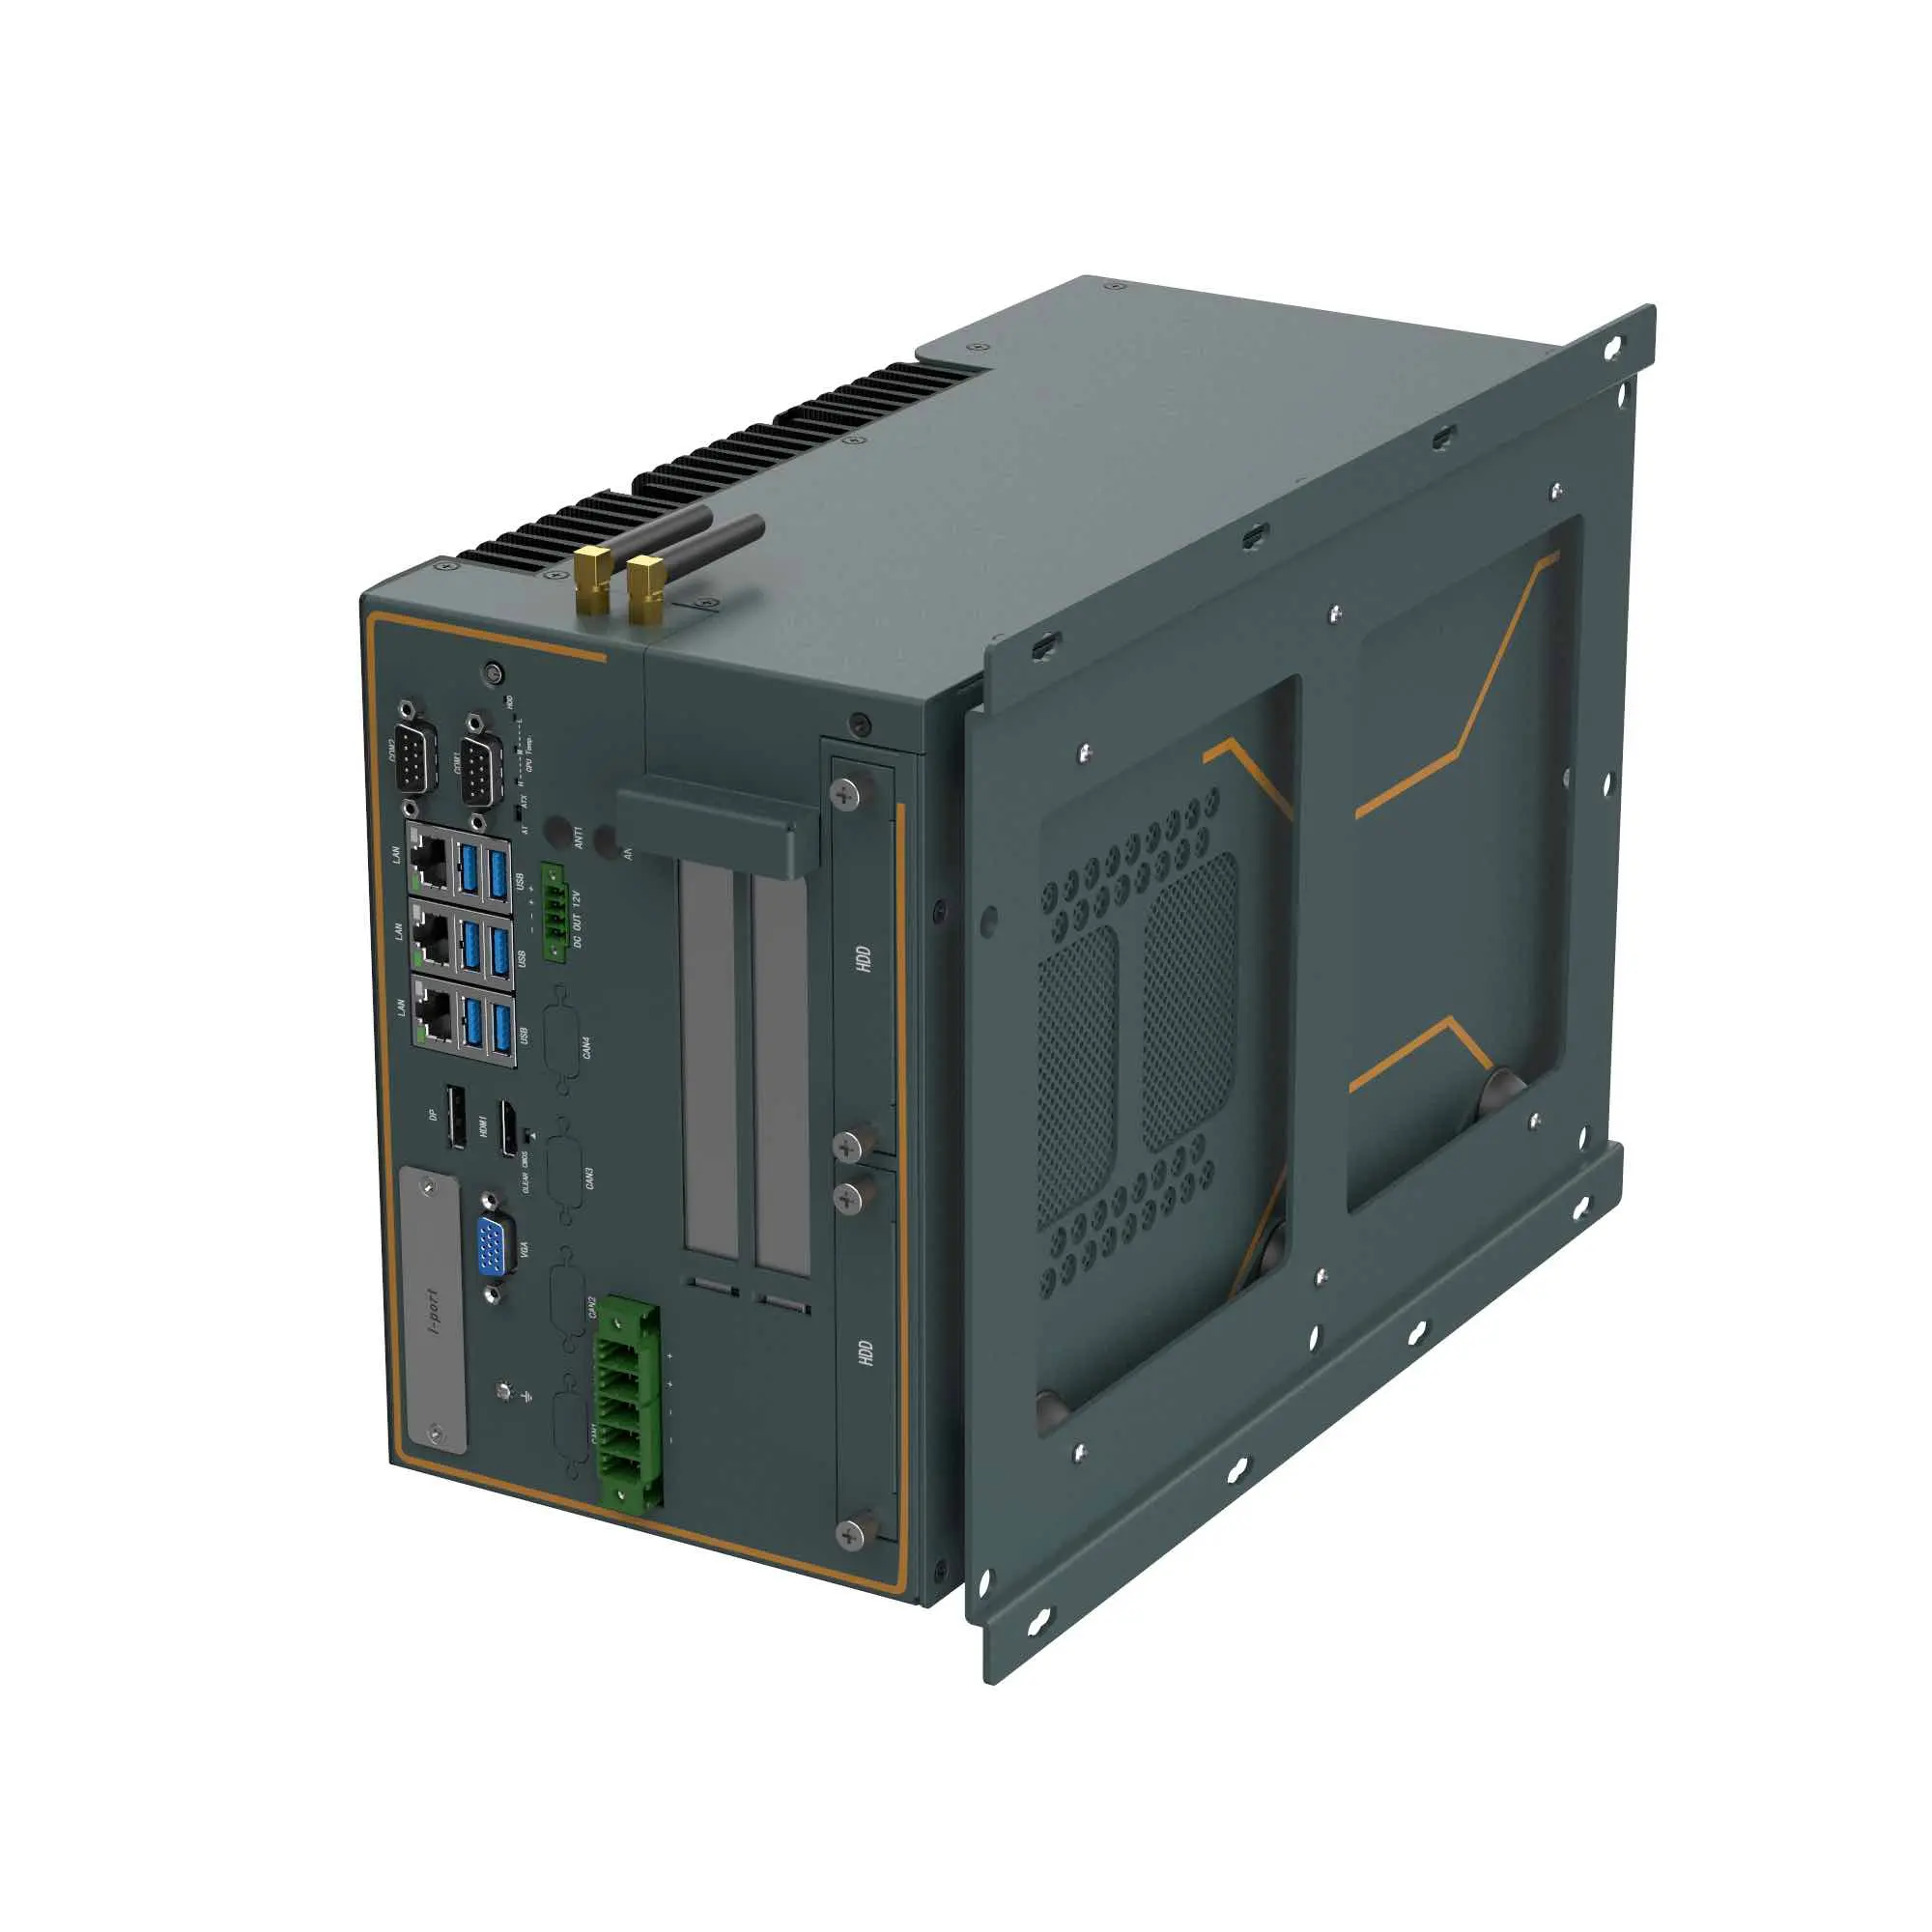
\includegraphics[width=0.4\textwidth]{gambar/brav7720.jpg}
    \caption{Komputer industrial BRAV-7720 (JHCTech) yang digunakan sebagai unit pemrosesan utama.}
    \label{fig:brav_computer}
\end{figure}

Komputasi dilakukan pada komputer industrial BRAV-7720 (JHCTech) tanpa kipas dengan prosesor Intel Core i7 generasi ke-12 dan GPU NVIDIA RTX 4060 (115 W, VRAM 8 GB).
Komputer ini menjalankan sistem operasi Ubuntu Linux dengan ROS2 sebagai kerangka kerja integrasi seluruh modul perangkat lunak.

\subsubsection{GPS u-blox ZED-F9P}

\begin{figure}[H]
    \centering
    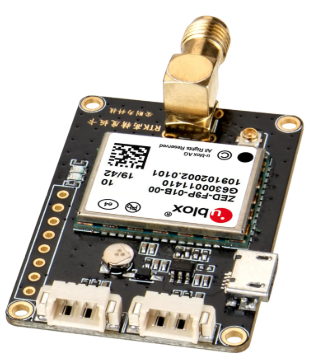
\includegraphics[width=0.3\textwidth]{gambar/ublox.png}
    \caption{Modul GPS u-blox ZED-F9P yang digunakan untuk data posisi global.}
    \label{fig:ublox_gps}
\end{figure}

Data posisi global diperoleh dari modul GNSS u-blox ZED-F9P yang mendukung konstelasi multi-satelit dan pita ganda (L1/L2).
Modul ini menyediakan data posisi dengan akurasi tingkat submeter melalui antarmuka UART ke komputer utama.
Data posisi digunakan sebagai masukan utama bagi modul lokalisasi dan sebagai rute titik acuan pada modul perencanaan global.

\subsubsection{IMU RION TL740D}

\begin{figure}[H]
    \centering
    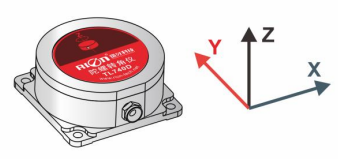
\includegraphics[width=0.6\textwidth]{gambar/rion.png}
    \caption{Sensor Inertial Measurement Unit (IMU) RION TL740D yang digunakan untuk data percepatan dan kecepatan sudut.}
    \label{fig:rion_imu}
\end{figure}

Sensor \emph{Inertial Measurement Unit} (IMU) RION TL740D digunakan untuk memperoleh data percepatan linear dan kecepatan sudut pada tiga sumbu.
Data IMU diintegrasikan ke dalam Kalman Filter sebagai masukan prediksi model dan digunakan untuk estimasi orientasi kendaraan.
Sensor ini juga menyediakan data 9 sumbu yang mencakup pitch, roll, yaw, percepatan pada tiga sumbu, dan kecepatan sudut pada tiga sumbu, sehingga memberikan informasi lengkap tentang dinamika kendaraan.

\subsubsection{Modul MKS CANable Pro}

\begin{figure}[H]
    \centering
    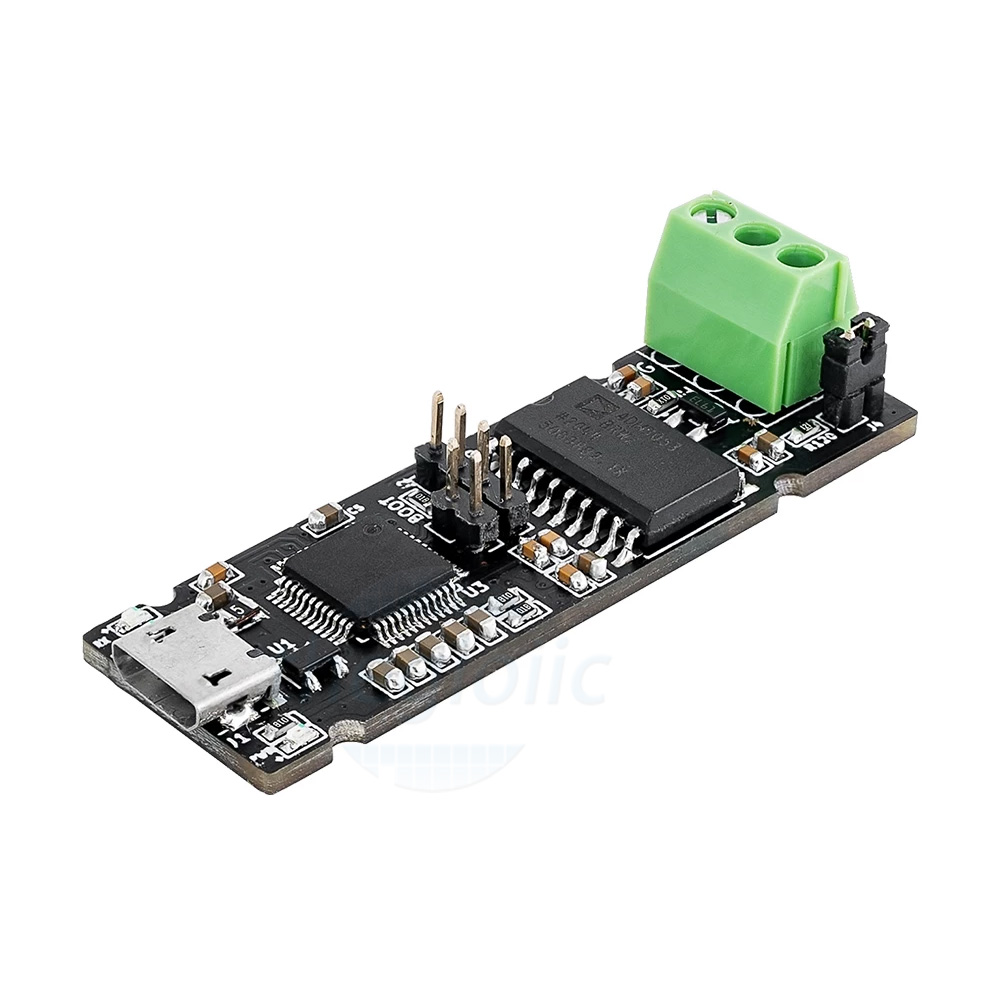
\includegraphics[width=0.4\textwidth]{gambar/mks-canable-pro.jpg}
    \caption{Modul MKS CANable Pro yang digunakan sebagai konverter CAN FD ke USB.}
    \label{fig:canable_pro}
\end{figure}

Modul MKS CANable Pro digunakan sebagai konverter CAN FD ke USB untuk menjembatani komunikasi antara komputer utama dengan jaringan CAN kendaraan.
Modul ini memungkinkan pengiriman data aktuator ke kendaraan dan data sensor odometri roda ke komputer utama untuk diproses lebih lanjut.
Selain itu, modul ini juga mendukung CAN FD dengan \emph{payload} hingga 64 bita per \emph{frame}.

\subsubsection{Ecoflow River 2 Pro}

\begin{figure}[H]
    \centering
    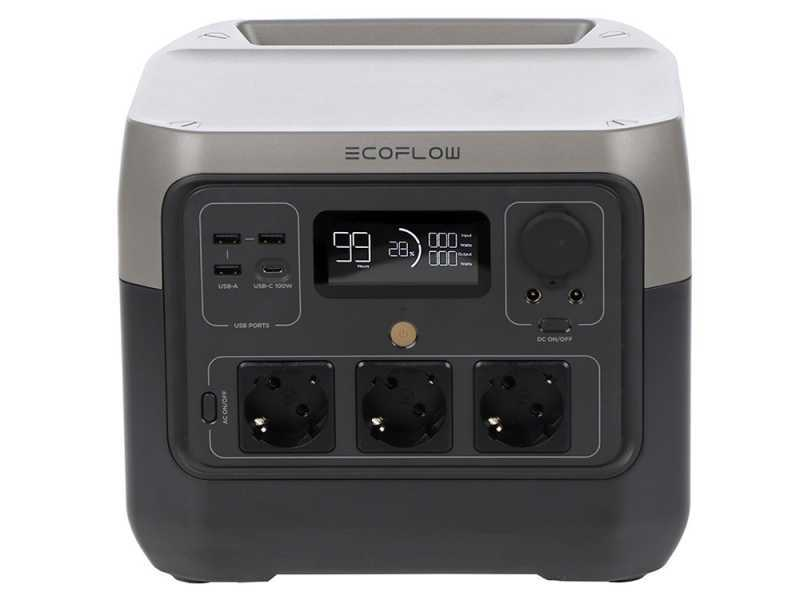
\includegraphics[width=0.4\textwidth]{gambar/ecoflow-river-2-pro.jpg}
    \caption{Power station portabel Ecoflow River 2 Pro yang digunakan untuk menyuplai daya selama pengujian lapangan.}
    \label{fig:ecoflow_power}
\end{figure}

Seluruh perangkat elektronik disuplai menggunakan \emph{power station} portabel Ecoflow River 2 Pro dengan kapasitas 768 Wh dan daya keluaran maksimum 1600 W.
Alat ini menyediakan port AC, DC, dan USB untuk menyuplai komputer, sensor, dan perangkat pendukung selama pengujian lapangan.

\subsection{Perangkat Lunak}

\begin{figure}[H]
    \centering
    
\includegraphics[width=0.6\textwidth]{gambar/ros2.png}
    \caption{Kerangka kerja ROS2 yang digunakan untuk integrasi perangkat lunak.}
    \label{fig:ros2_framework}
\end{figure}

Seluruh modul perangkat lunak diimplementasikan dalam kerangka kerja ROS2 (\emph{Robot Operating System 2}) yang berjalan pada sistem operasi Ubuntu Linux 22.04.
ROS2 menyediakan infrastruktur komunikasi antar modul melalui \emph{topics}, \emph{services}, dan \emph{actions}, serta mendukung integrasi dengan berbagai pustaka pemrosesan citra, algoritma fusi sensor, dan perencanaan lintasan.
Dengan menggunakan ROS2, integrasi antara segmentasi visual, fusi sensor Kalman Filter, dan perencanaan lintasan dapat dilakukan secara modular dan terstruktur, memudahkan pengembangan dan pengujian sistem navigasi kendaraan otonom ini.



\subsection{Alat Ukur}

Pengukuran data aktual posisi dilakukan menggunakan pita ukur dengan ketelitian 0,5 mm sebagai penanda titik acuan pada lintasan uji.
Waktu tempuh kendaraan antar titik acuan diukur menggunakan \emph{stopwatch} untuk memperoleh data waktu aktual yang digunakan sebagai referensi dalam perhitungan RMSE posisi dan kecepatan.
